% Options for packages loaded elsewhere
\PassOptionsToPackage{unicode}{hyperref}
\PassOptionsToPackage{hyphens}{url}
%
\documentclass[
  ignorenonframetext,
  aspectratio=169,
]{beamer}
\usepackage{pgfpages}
\setbeamertemplate{caption}[numbered]
\setbeamertemplate{caption label separator}{: }
\setbeamertemplate{navigation symbols}{}
\setbeamertemplate{footline}[page number]
\setbeamertemplate{itemize item}{\small\raise0.5pt\hbox{$\bullet$}}
\setbeamertemplate{itemize subitem}{\tiny\raise1.5pt\hbox{$\bullet$}}
\setbeamertemplate{itemize subsubitem}{\tiny\raise1.5pt\hbox{$\bullet$}}
\setbeamercolor{caption name}{fg=normal text.fg}
\beamertemplatenavigationsymbolsempty
% Prevent slide breaks in the middle of a paragraph
\widowpenalties 1 10000
\raggedbottom
\setbeamertemplate{part page}{
  \centering
  \begin{beamercolorbox}[sep=16pt,center]{part title}
    \usebeamerfont{part title}\insertpart\par
  \end{beamercolorbox}
}
\setbeamertemplate{section page}{
  \centering
  \begin{beamercolorbox}[sep=12pt,center]{part title}
    \usebeamerfont{section title}\insertsection\par
  \end{beamercolorbox}
}
\setbeamertemplate{subsection page}{
  \centering
  \begin{beamercolorbox}[sep=8pt,center]{part title}
    \usebeamerfont{subsection title}\insertsubsection\par
  \end{beamercolorbox}
}
\AtBeginPart{
  \frame{\partpage}
}
\AtBeginSection{
  \ifbibliography
  \else
    \frame{\sectionpage}
  \fi
}
\AtBeginSubsection{
  \frame{\subsectionpage}
}
\usepackage{amsmath,amssymb}
\usepackage{lmodern}
\usepackage{iftex}
\ifPDFTeX
  \usepackage[T1]{fontenc}
  \usepackage[utf8]{inputenc}
  \usepackage{textcomp} % provide euro and other symbols
\else % if luatex or xetex
  \ifXeTeX
    \usepackage{xltxtra} 
    \usepackage{xeCJK}
    \setCJKmainfont{ipaexm.ttf}
    \setCJKsansfont{ipaexg.ttf}
    \setCJKmonofont{ipaexg.ttf}
  \fi
  \usepackage{unicode-math}
  \defaultfontfeatures{Scale=MatchLowercase}
  \defaultfontfeatures[\rmfamily]{Ligatures=TeX,Scale=1}
\fi
% Use upquote if available, for straight quotes in verbatim environments
\IfFileExists{upquote.sty}{\usepackage{upquote}}{}
\IfFileExists{microtype.sty}{% use microtype if available
  \usepackage[]{microtype}
  \UseMicrotypeSet[protrusion]{basicmath} % disable protrusion for tt fonts
}{}
\makeatletter
\@ifundefined{KOMAClassName}{% if non-KOMA class
  \IfFileExists{parskip.sty}{%
    \usepackage{parskip}
  }{% else
    \setlength{\parindent}{0pt}
    \setlength{\parskip}{6pt plus 2pt minus 1pt}}
}{% if KOMA class
  \KOMAoptions{parskip=half}}
\makeatother
\usepackage{xcolor}
\IfFileExists{xurl.sty}{\usepackage{xurl}}{} % add URL line breaks if available
\IfFileExists{bookmark.sty}{\usepackage{bookmark}}{\usepackage{hyperref}}
\hypersetup{
  pdftitle={Estimating Effect of Tax Incentives on Charitable Giving Considering Self-Selection of Tax Relief in South Korea},
  hidelinks,
  pdfcreator={LaTeX via pandoc}}
\urlstyle{same} % disable monospaced font for URLs

\usepackage{setspace}
\usepackage{float}

\newif\ifbibliography
\usepackage{longtable,booktabs,array}
\usepackage{threeparttable, threeparttablex, multirow}
\usepackage{calc} % for calculating minipage widths
\usepackage{caption}
% Make caption package work with longtable
\makeatletter
\def\fnum@table{\tablename~\thetable}
\makeatother
\usepackage{graphicx}
\makeatletter
\def\maxwidth{\ifdim\Gin@nat@width>\linewidth\linewidth\else\Gin@nat@width\fi}
\def\maxheight{\ifdim\Gin@nat@height>\textheight\textheight\else\Gin@nat@height\fi}
\makeatother
% Scale images if necessary, so that they will not overflow the page
% margins by default, and it is still possible to overwrite the defaults
% using explicit options in \includegraphics[width, height, ...]{}
\setkeys{Gin}{width=\maxwidth,height=\maxheight,keepaspectratio}
% Set default figure placement to htbp
\makeatletter
\def\fps@figure{htbp}
\makeatother
\setlength{\emergencystretch}{3em} % prevent overfull lines
\providecommand{\tightlist}{%
  \setlength{\itemsep}{0pt}\setlength{\parskip}{0pt}}
\setcounter{secnumdepth}{-\maxdimen} % remove section numbering
\newlength{\cslhangindent}
\setlength{\cslhangindent}{1.5em}
\newlength{\csllabelwidth}
\setlength{\csllabelwidth}{3em}
\newlength{\cslentryspacingunit} % times entry-spacing
\setlength{\cslentryspacingunit}{\parskip}
\newenvironment{CSLReferences}[2] % #1 hanging-ident, #2 entry spacing
 {% don't indent paragraphs
  \setlength{\parindent}{0pt}
  % turn on hanging indent if param 1 is 1
  \ifodd #1
  \let\oldpar\par
  \def\par{\hangindent=\cslhangindent\oldpar}
  \fi
  % set entry spacing
  \setlength{\parskip}{#2\cslentryspacingunit}
 }%
 {}
\usepackage{calc}
\newcommand{\CSLBlock}[1]{#1\hfill\break}
\newcommand{\CSLLeftMargin}[1]{\parbox[t]{\csllabelwidth}{#1}}
\newcommand{\CSLRightInline}[1]{\parbox[t]{\linewidth - \csllabelwidth}{#1}\break}
\newcommand{\CSLIndent}[1]{\hspace{\cslhangindent}#1}


\ifLuaTeX
  \usepackage{selnolig}  % disable illegal ligatures
\fi

\title{Estimating Effect of Tax Incentives on Charitable Giving Considering Self-Selection of Tax Relief in South Korea  }
\author[shortname]{ Hiroki Kato \inst{1} \and  Tsuyoshi Goto \inst{2} \and  Yong-Rok Kim \inst{3} \and }
\institute[shortinst]{ \inst{1} Osaka University \and  \inst{2} Chiba University \and  \inst{3} Kansai University \and }

\date{2021/12/27}


\begin{document}
\frame{\titlepage}

\begin{frame}
\end{frame}

\hypertarget{data}{%
\section{Data}\label{data}}

\begin{frame}{National Survey of Tax and Benefit (NaSTaB)}
\protect\hypertarget{national-survey-of-tax-and-benefit-nastab}{}
\begin{itemize}
\tightlist
\item
  NaSTaB has been implemented by The Korea Institute of Taxation and Finance since 2008
\item
  The NaSTaB is an annual panel data on households' tax burden and public benefits
\item
  The unit of analysis is 5,634 households throughout the country

  \begin{itemize}
  \tightlist
  \item
    5,634 family heads and family members with more than 15 years old and with income or economically active
  \end{itemize}
\item
  Our analysis uses the NaSTaB data from (i) 2013-2018 and (ii) excluding respondents under the age of 23.

  \begin{itemize}
  \tightlist
  \item
    using the NaSTaB data before 2012 captures the effects of other tax reform than the reform in 2014.
  \item
    we exclude respondents whose age is under 23 because they are not likely to have income or assets.
  \end{itemize}
\end{itemize}
\end{frame}

\begin{frame}{Descriptive Statistics}
\protect\hypertarget{descriptive-statistics}{}
\begin{table}

\caption{\label{tab:SummaryCovariate}Descriptive Statistics}
\centering
\fontsize{6}{8}\selectfont
\begin{tabular}[t]{lcccccc}
\toprule
  & N & Mean & Std.Dev. & Min & Median & Max\\
\midrule
\addlinespace[0.3em]
\multicolumn{7}{l}{\textbf{Income and giving price}}\\
\hspace{1em}Annual taxable labor income (unit: 10,000KRW) & 36189 & 1747.26 & 2696.77 & 0.00 & 0.00 & 50000.00\\
\hspace{1em}First giving relative price & 36198 & 0.86 & 0.04 & 0.62 & 0.85 & 0.94\\
\addlinespace[0.3em]
\multicolumn{7}{l}{\textbf{Charitable giving}}\\
\hspace{1em}Annual chariatable giving (unit: 10,000KRW) & 36199 & 35.64 & 153.20 & 0.00 & 0.00 & 10000.00\\
\hspace{1em}Dummary of donation > 0 & 36199 & 0.24 & 0.42 & 0.00 & 0.00 & 1.00\\
\hspace{1em}Dummy of declaration of a tax relief & 36199 & 0.10 & 0.30 & 0.00 & 0.00 & 1.00\\
\addlinespace[0.3em]
\multicolumn{7}{l}{\textbf{Individual Characteristics}}\\
\hspace{1em}Age & 36199 & 53.45 & 16.22 & 24.00 & 51.00 & 103.00\\
\hspace{1em}Female dummy & 36199 & 0.43 & 0.50 & 0.00 & 0.00 & 1.00\\
\hspace{1em}University graduate & 36198 & 0.42 & 0.49 & 0.00 & 0.00 & 1.00\\
\hspace{1em}High school graduate dummy & 36198 & 0.31 & 0.46 & 0.00 & 0.00 & 1.00\\
\hspace{1em}Junior high school graduate dummy & 36198 & 0.27 & 0.44 & 0.00 & 0.00 & 1.00\\
\hspace{1em}Wage earner dummy & 27394 & 0.56 & 0.50 & 0.00 & 1.00 & 1.00\\
\hspace{1em}\#.Tax accountant / population & 36199 & 1.04 & 0.51 & 0.32 & 0.92 & 2.24\\
\bottomrule
\end{tabular}
\end{table}
\end{frame}

\begin{frame}{Right-Skewed Income Distribution and Price Variation for Identification}
\protect\hypertarget{right-skewed-income-distribution-and-price-variation-for-identification}{}
\begin{figure}[t]

{\centering 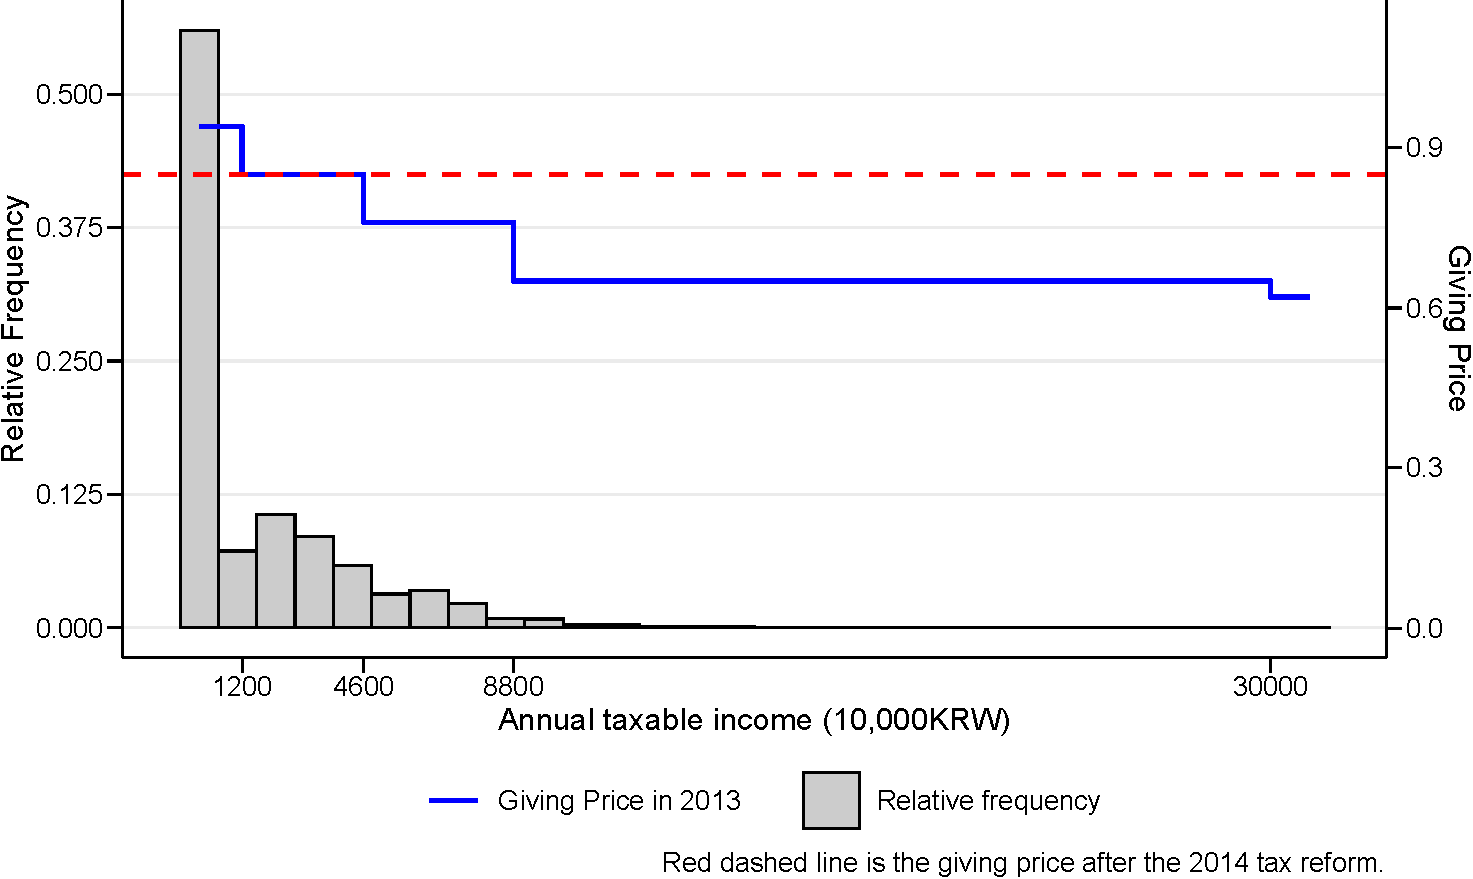
\includegraphics[width=0.7\linewidth,]{C:/Users/katoo/Desktop/NASTAB/paper/slide_files/figure-beamer/SummaryPrice-1} 

}

\caption{Income Distribution in 2013 and Relative Giving Price. Notes: The left and right axis measure the relative frequency of respondents (grey bars) and the relative giving price (solid step line and dashed line), respectively. A solid step line and a dashed horizontal line represents the giving price in 2013 and 2014, respectively.}\label{fig:SummaryPrice}
\end{figure}
\end{frame}

\begin{frame}{Message from Figure \ref{fig:SummaryPrice}}
\protect\hypertarget{message-from-figure-reffigsummaryprice}{}
Right-skewed income distribution:

\begin{itemize}
\tightlist
\item
  NaSTaB contains the annual taxable labor income last year
\item
  Our sample includes subjects with no labor income (e.g.~housewives)

  \begin{itemize}
  \tightlist
  \item
    Table \ref{tab:SummaryCovariate}: the average income is 17.54 million KRW
  \end{itemize}
\item
  National Tax Statistical Yearbook 2012-2018 (Korean National Tax Service): the average annual taxable income is 32.77 million KRW

  \begin{itemize}
  \tightlist
  \item
    Sample: employees who submitted the tax return
  \end{itemize}
\end{itemize}

Price variation for indetification

\begin{itemize}
\tightlist
\item
  Based on changes in tax incentive due to the 2014 tax reform, we can devide into three income groups:

  \begin{enumerate}
  \tightlist
  \item
    less than 120 million KRW: expanded tax incentive (decreased giving price)
  \item
    between 120 million KRW and 460 million KRW: unchanged tax incentive
  \item
    more than 460 million KRW: decreased tax incentive (increaed giving price)
  \end{enumerate}
\item
  This is main source of identification for effect of tax incentive on giving.
\end{itemize}
\end{frame}

\begin{frame}{Donors Decreased Immediately After Tax Reform}
\protect\hypertarget{donors-decreased-immediately-after-tax-reform}{}
\begin{figure}[t]

{\centering 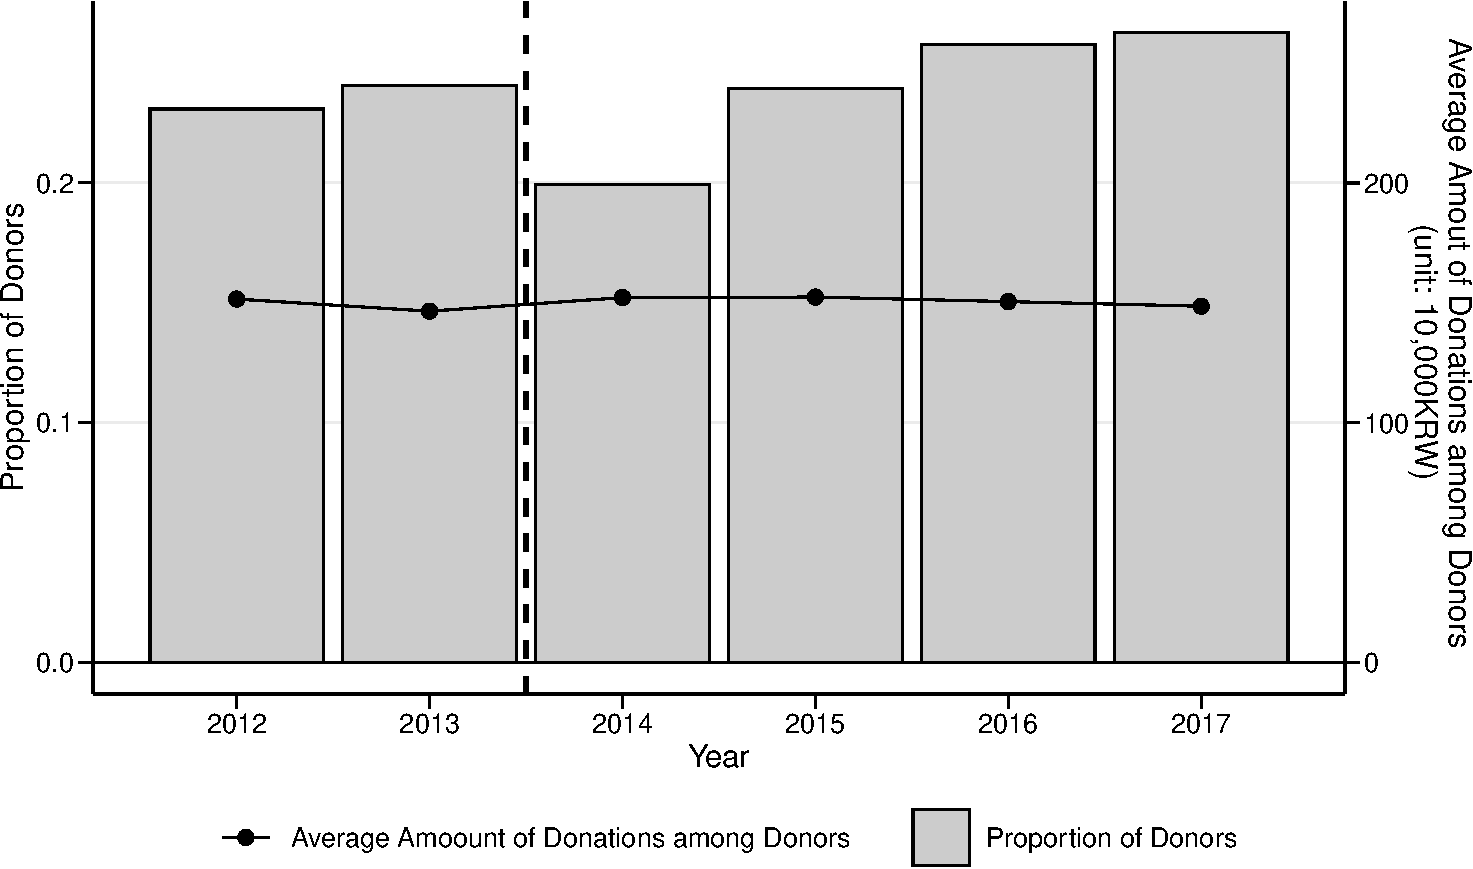
\includegraphics[width=0.7\linewidth,]{C:/Users/katoo/Desktop/NASTAB/paper/slide_files/figure-beamer/SummaryGiving-1} 

}

\caption{Proportion of Donors and Average Donations among Donors. Notes: The left and right axises measure prooortion of donors (grey bars) and the average amount of donations among donors (solid line), respectively.}\label{fig:SummaryGiving}
\end{figure}
\end{frame}

\begin{frame}{Message from Figure \ref{fig:SummaryGiving}}
\protect\hypertarget{message-from-figure-reffigsummarygiving}{}
\begin{itemize}
\tightlist
\item
  Proportion of donors across years: 24\% (Table \ref{tab:SummaryCovariate})
\item
  2014: Proportion of donors is lower than before the tax reform

  \begin{itemize}
  \tightlist
  \item
    After that, proportion of donors has continued to increase, finally surpassing that before the tax reform
  \end{itemize}
\end{itemize}

Notes:

\begin{itemize}
\tightlist
\item
  average donation conditional on donors has been stable across year

  \begin{itemize}
  \tightlist
  \item
    1.5 million KRW (7\% of average income)
  \item
    Table \ref{tab:SummaryCovariate}: Unconditional average donation is 358,600 KRW (2\% of average income)
  \end{itemize}
\end{itemize}
\end{frame}

\begin{frame}{Price Effect Can Be Observed}
\protect\hypertarget{price-effect-can-be-observed}{}
\begin{figure}[t]

{\centering 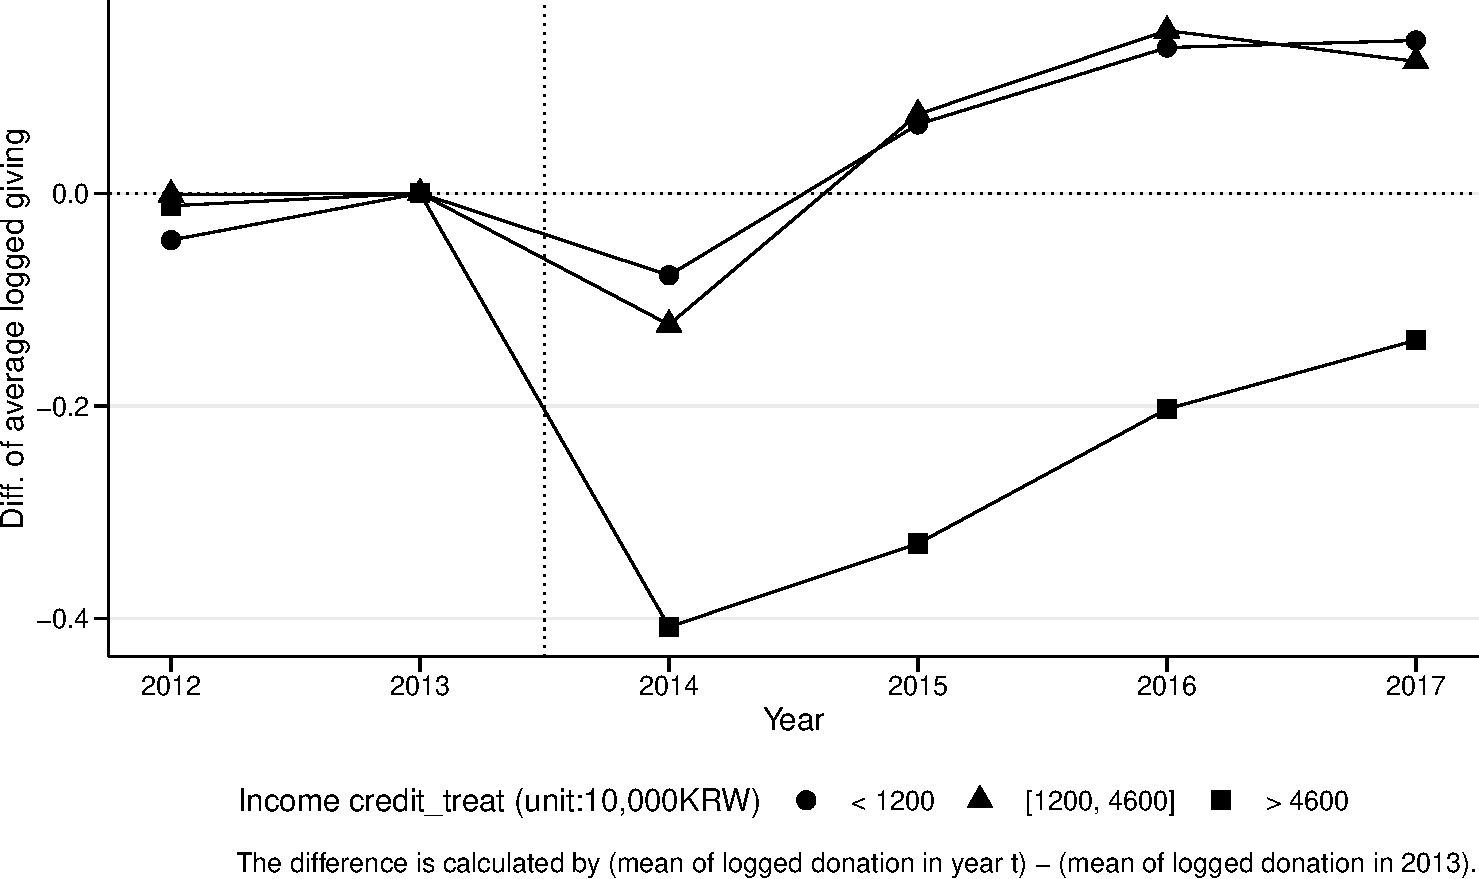
\includegraphics[width=0.7\linewidth,]{C:/Users/katoo/Desktop/NASTAB/paper/slide_files/figure-beamer/SummaryGivingOverall-1} 

}

\caption{Average Logged Giving by Three Income Groups. Notes: We created three income groups, with the relative price of giving rising (circle), unchanged (triangle), and falling (square) between 2013 and 2014. The group averages are normalized to be zero in 2013.}\label{fig:SummaryGivingOverall}
\end{figure}
\end{frame}

\begin{frame}{Message from Figure \ref{fig:SummaryGivingOverall}}
\protect\hypertarget{message-from-figure-reffigsummarygivingoverall}{}
Price effect = Tax incentive increases charitable giving

\begin{itemize}
\tightlist
\item
  Donations for income groups with unchanged or increased tax incentives have exceeded those in 2013 since 2015
\item
  Donations for income groups with reduced tax incentives have been lower than before tax reform since 2015
\end{itemize}

Other findings:

\begin{enumerate}
\tightlist
\item
  Prior to the 2014 tax reform, donations did not change in all groups
\item
  Donations for all groups were lower than in 2013

  \begin{itemize}
  \tightlist
  \item
    Donations for income groups with reduced tax incentive due to the 2014 tax reform was 40\% of that in 2013
  \item
    Announcement effect? Learning effect?
  \end{itemize}
\end{enumerate}
\end{frame}

\begin{frame}{Price Effect Can Be Partially Observed for Intensive Margin}
\protect\hypertarget{price-effect-can-be-partially-observed-for-intensive-margin}{}
\begin{figure}[t]

{\centering 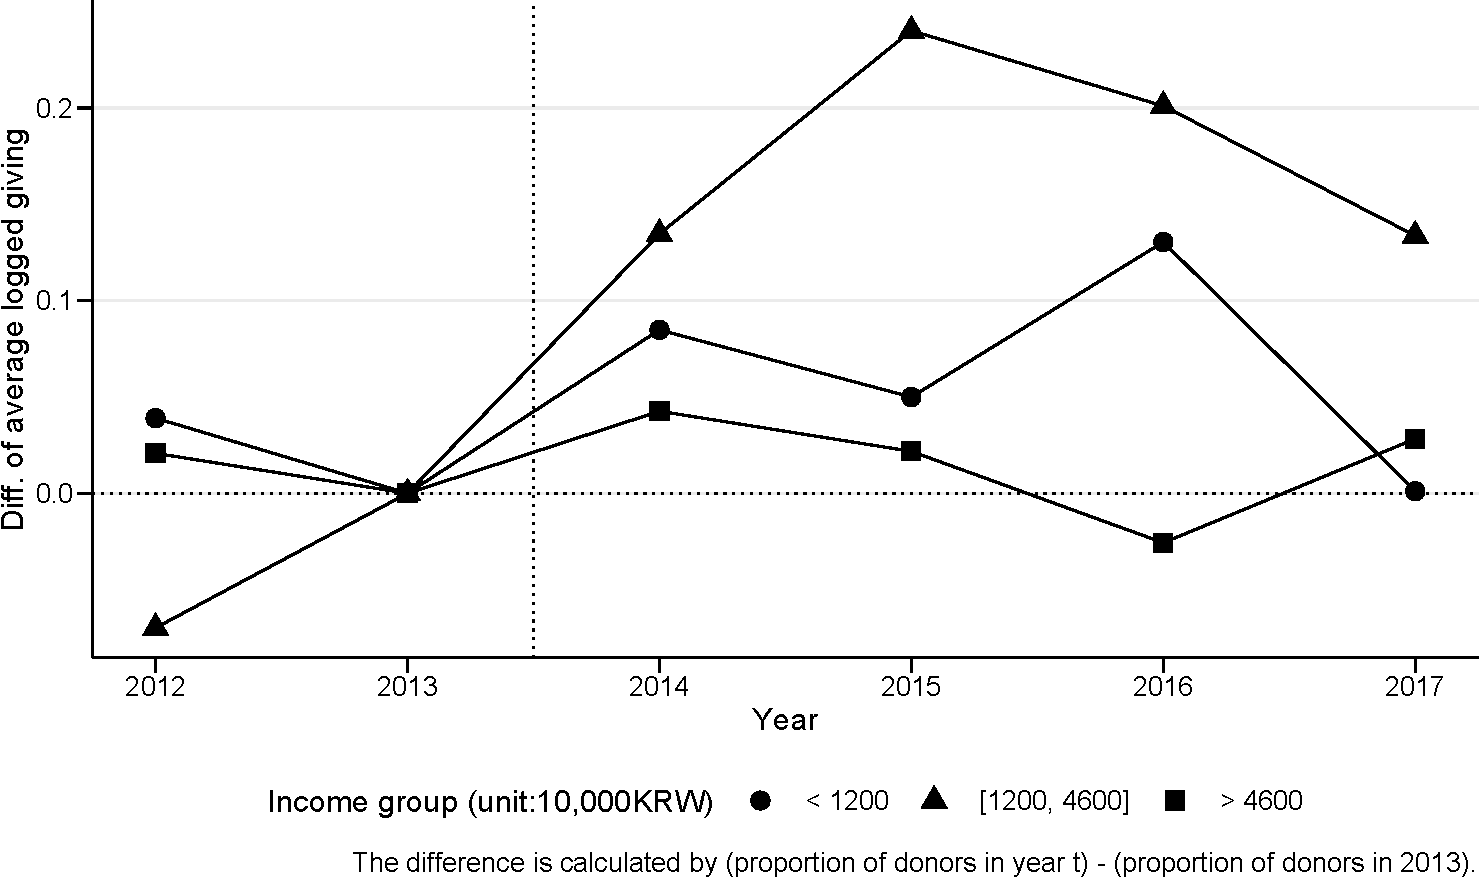
\includegraphics[width=0.7\linewidth,]{C:/Users/katoo/Desktop/NASTAB/paper/slide_files/figure-beamer/SummaryGivingIntensive-1} 

}

\caption{Average Logged Giving by Three Income Groups Conditional on Donors. Notes: We created three income groups, with the relative price of giving rising (circle), unchanged (triangle), and falling (square) between 2013 and 2014. The group averages are normalized to be zero in 2013.}\label{fig:SummaryGivingIntensive}
\end{figure}
\end{frame}

\begin{frame}{Price Effect Can Be Observed for Extensive Margin}
\protect\hypertarget{price-effect-can-be-observed-for-extensive-margin}{}
\begin{figure}[t]

{\centering 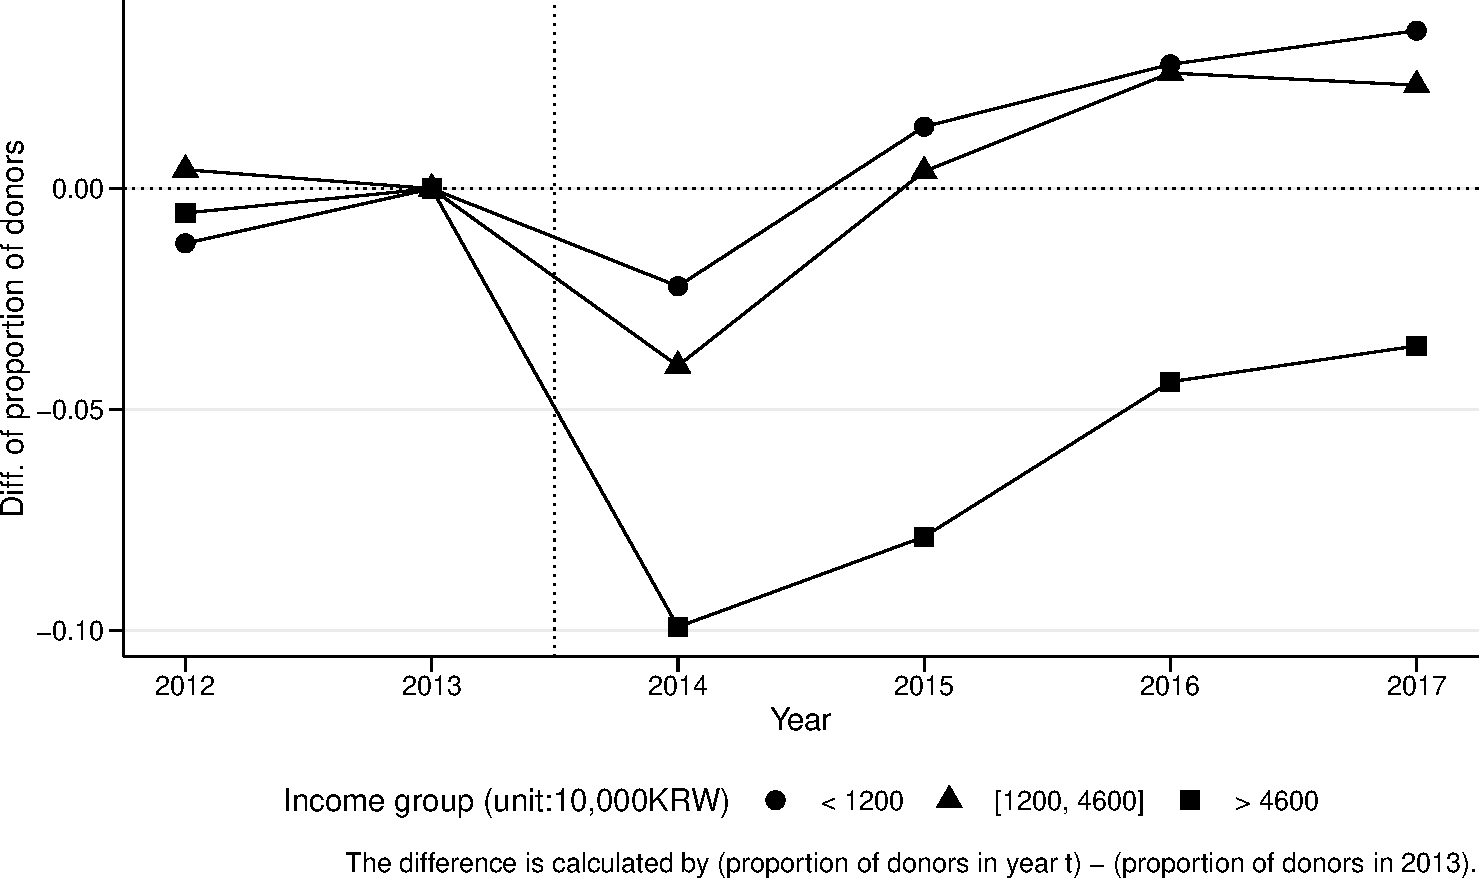
\includegraphics[width=0.7\linewidth,]{C:/Users/katoo/Desktop/NASTAB/paper/slide_files/figure-beamer/SummaryGivingExtensive-1} 

}

\caption{Proportion of Donors by Three Income Groups. Notes: We created three income groups, with the relative price of giving rising (circle), unchanged (triangle), and falling (square) between 2013 and 2014. The group averages are normalized to be zero in 2013.}\label{fig:SummaryGivingExtensive}
\end{figure}
\end{frame}

\begin{frame}{Message from Figure \ref{fig:SummaryGivingIntensive} and \ref{fig:SummaryGivingExtensive}}
\protect\hypertarget{message-from-figure-reffigsummarygivingintensive-and-reffigsummarygivingextensive}{}
Intensive margin (How much donors give): Price effect can be partially observed

\begin{itemize}
\tightlist
\item
  The income group that increased the donation most was the group whose tax incentive did not change, but the donation of the income group that decreased the tax incentive did not change significantly.
\item
  Income groups with unchanged tax incentives has increased donations more than income groups with expanded tax incentives (opposite to the price effect).
\end{itemize}

Extensive margin (Whethre respondents donate): Price effect can be observed

\begin{itemize}
\tightlist
\item
  Same trend as Figure \ref{fig:SummaryGivingOverall}
\end{itemize}
\end{frame}

\begin{frame}{Application for Tax Relief Decreased After Tax Reform}
\protect\hypertarget{application-for-tax-relief-decreased-after-tax-reform}{}
\begin{figure}[t]

{\centering 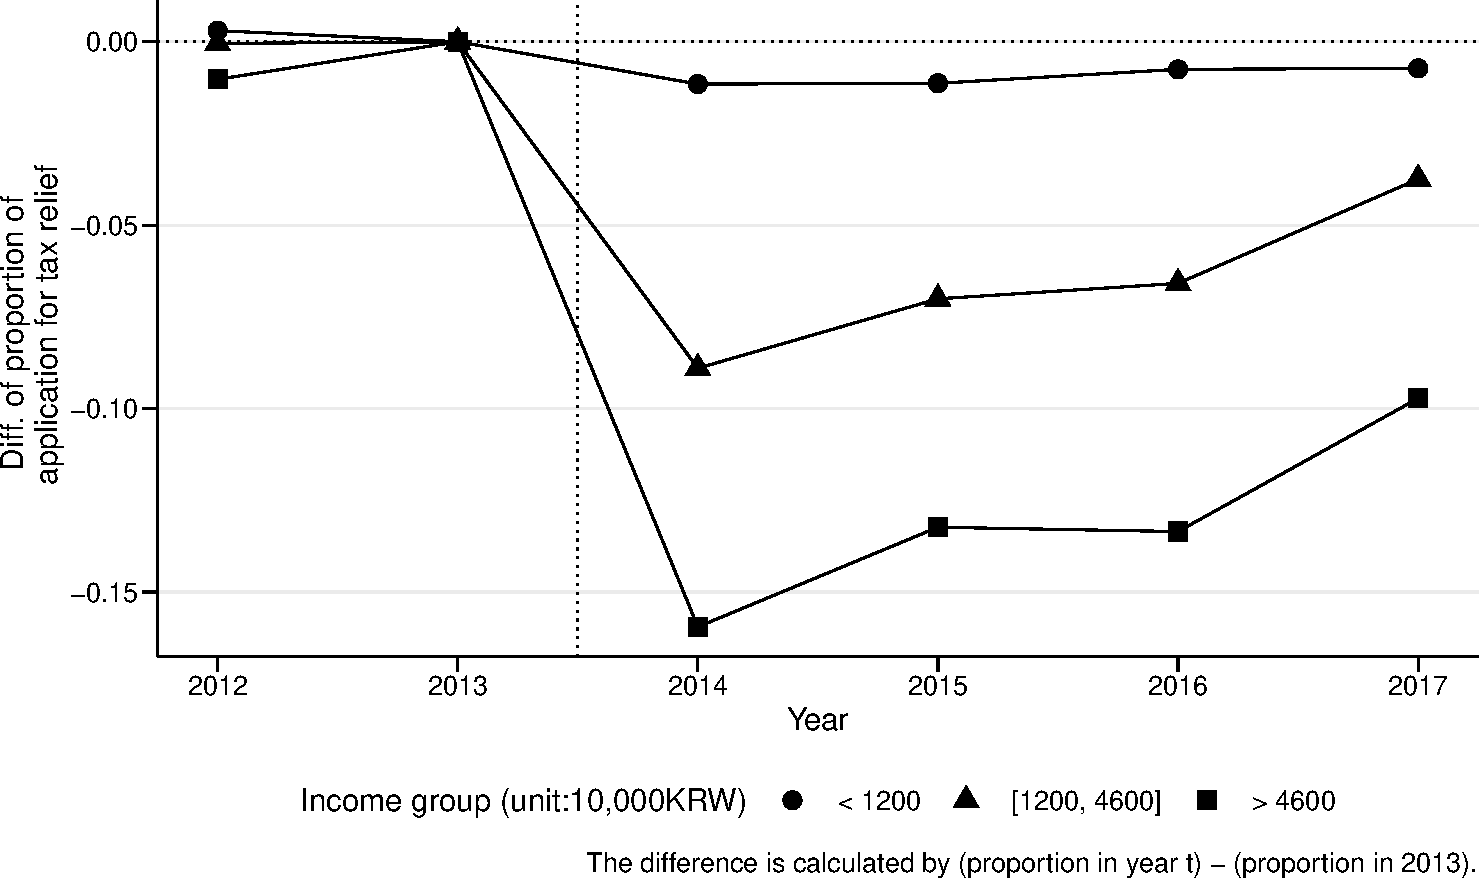
\includegraphics[width=0.7\linewidth,]{C:/Users/katoo/Desktop/NASTAB/paper/slide_files/figure-beamer/SummaryReliefbyIncome-1} 

}

\caption{Proportion of Having Applied for Tax Relief by Three Income Groups. Notes: We created three income groups, with the relative price of giving rising (circle), unchanged (triangle), and falling (square) between 2013 and 2014. The group averages are normalized to be zero in 2013.}\label{fig:SummaryReliefbyIncome}
\end{figure}
\end{frame}

\begin{frame}{Message from Figure \ref{fig:SummaryReliefbyIncome}}
\protect\hypertarget{message-from-figure-reffigsummaryreliefbyincome}{}
\begin{enumerate}
\tightlist
\item
  tax incentive negatively correlated with application for tax relief.

  \begin{itemize}
  \tightlist
  \item
    Since the 2014 tax reform, the share of application for tax relief has not increased in all income groups compared to 2013.
  \item
    the decrease in the application rate is the largest among income groups whose tax incentives decreased due to the 2014 tax reform.
  \end{itemize}
\item
  the trend of application for tax relief does not match the trend of share of donors.

  \begin{itemize}
  \tightlist
  \item
    If there is no application cost, all donors should apply for tax relief
  \item
    Figure \ref{fig:SummaryGivingExtensive} and \ref{fig:SummaryReliefbyIncome} imply that there is cost to apply for tax relief.
  \item
    The distribution of donations conditional on donors does not change significantly depending on whether or not they have applied for tax relief, suggesting that the application cost is high (Figure \ref{fig:SummaryGivingIntensiveDist}).
  \end{itemize}
\end{enumerate}
\end{frame}

\begin{frame}{Wage Earners Are More Likely to Apply for Tax Relief}
\protect\hypertarget{wage-earners-are-more-likely-to-apply-for-tax-relief}{}
\begin{figure}[t]

{\centering 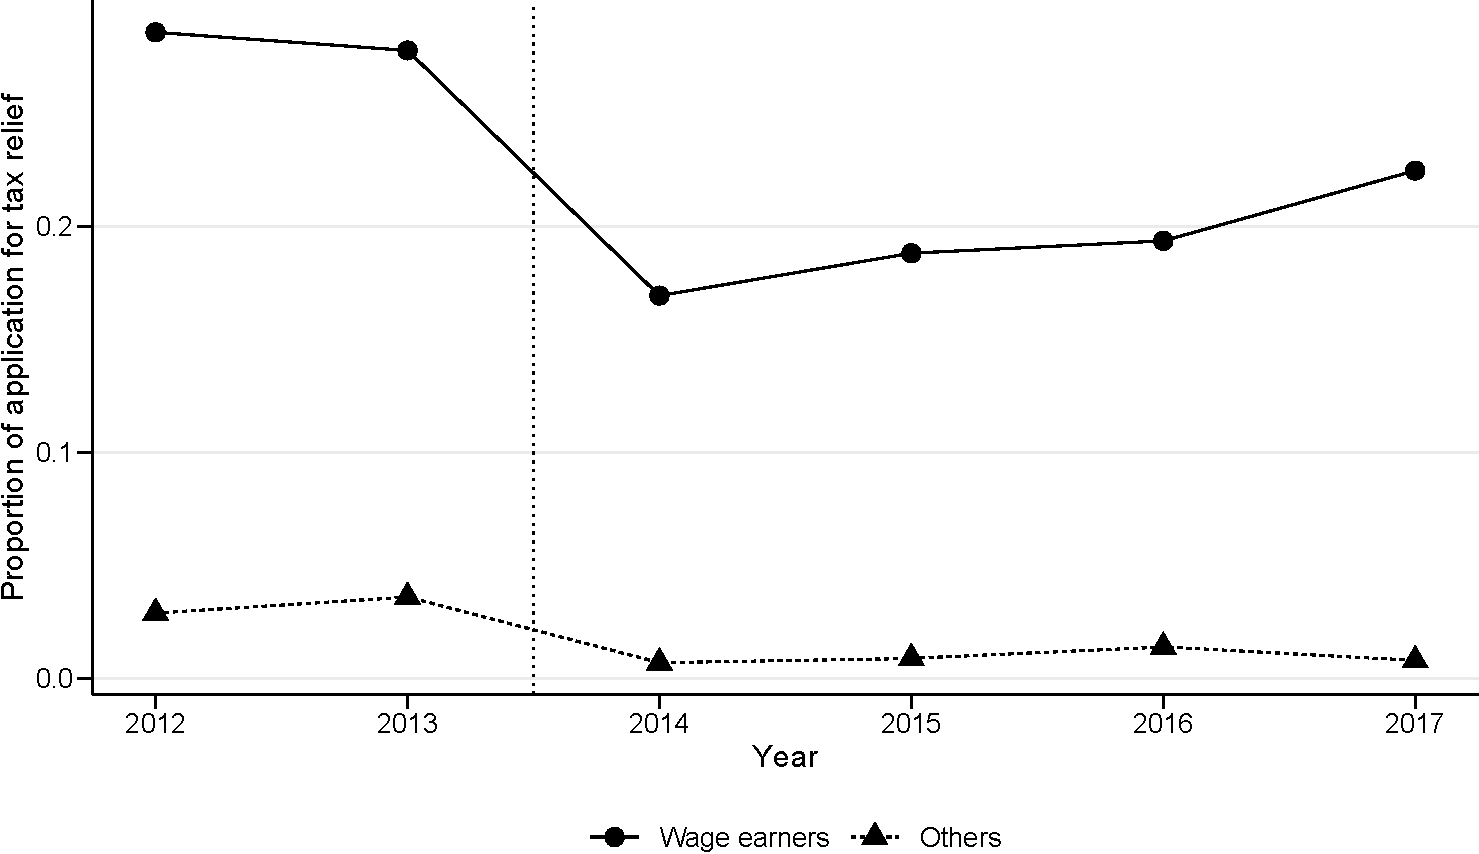
\includegraphics[width=0.7\linewidth,]{C:/Users/katoo/Desktop/NASTAB/paper/slide_files/figure-beamer/SummaryReliefbyEarner-1} 

}

\caption{Share of Tax Relief by Wage Earners. Notes: A solid line is the share of applying for tax relief among wage eaners. A dashed line is the share of applying for tax relief other than wage earners.}\label{fig:SummaryReliefbyEarner}
\end{figure}
\end{frame}

\begin{frame}{Message from Figure \ref{fig:SummaryReliefbyEarner}}
\protect\hypertarget{message-from-figure-reffigsummaryreliefbyearner}{}
\begin{itemize}
\tightlist
\item
  Employment status is one dimension of variation of applied cost.

  \begin{itemize}
  \tightlist
  \item
    self-employed workers have to retain the certificate until they submit tax return.
  \item
    wage earners can declare tax relief and submit the certificate through their company at any time.
  \end{itemize}
\item
  the proportion of declaring a tax relief among wage earners is higher than the others

  \begin{itemize}
  \tightlist
  \item
    Application cost for wage earners is lower than for other than wage earners
  \item
    This trend does not change when we calculate the proportion of application conditional on donors (Figure \ref{fig:SummaryReliefbyEarner2}).
  \end{itemize}
\end{itemize}
\end{frame}

\hypertarget{estimating-conventional-price-elasticities}{%
\section{Estimating Conventional Price Elasticities}\label{estimating-conventional-price-elasticities}}

\begin{frame}{Emprical Strategies}
\protect\hypertarget{emprical-strategies}{}
\begin{itemize}
\tightlist
\item
  We start to esimate the effect of tax incentive by estimating the price elasticity of charitable giving
\item
  Following Almunia et al. (2020), we estimate two types of elasticities: the intensive-margin price elasticity and the extensive-margin price elasticity

  \begin{itemize}
  \tightlist
  \item
    The intensive-margin price elasticity: how much a 1\% increase of price increases the amount of donations conditional on donors.
  \item
    The extensive-margin price elasticity: how much the probability of donating increases with a 1\% increase of price.
  \end{itemize}
\end{itemize}
\end{frame}

\begin{frame}{Estimation Equation for Intensive-Margin Elasticity}
\protect\hypertarget{estimation-equation-for-intensive-margin-elasticity}{}
\begin{align}
  \ln g_{it} = \theta_i + \gamma \ln p_t(y_{it}, R_{it}, g_{it})
  + \beta X_{it} + \lambda_t + u_{it}, \label{eq:intensive}
\end{align}

\begin{itemize}
\tightlist
\item
  \(X_{it}\) is a vector of covariate including income \(y_{it}\)
\item
  \(\theta_i\) is an individual fixed effect, and \(\lambda_t\) is a time fixed effect
\item
  \(u_{it}\) is an idiosyncratic error
\item
  Our prameter of interest is \(\gamma\), which represents the intensive-margin price elasticity.
\end{itemize}
\end{frame}

\begin{frame}{Estimation Equation for Extensive-Margin Elasticity}
\protect\hypertarget{estimation-equation-for-extensive-margin-elasticity}{}
\begin{align}
  D_{it} = \theta_i + \delta \ln p_t(y_{it}, R_{it}, g_{it})
  + \beta X_{it} + \lambda_t + u_{it}, \label{eq:extensive}
\end{align}

\begin{itemize}
\tightlist
\item
  \(D_{it}\) is a dummy taking one if positive giving is observed (\(g_{it} > 0\)).
\item
  Our prameter of interest is \(\delta\)

  \begin{itemize}
  \tightlist
  \item
    We cannot interpret the parameter \(\delta\) as the extensive-margin price elasticity beucase the outcome is a dummy variable.
  \item
    the extensive-maring price elasticity can be calculated as \(\hat{\delta} / \bar{D}\) where \(\bar{D}\) is sample mean of \(D_{it}\).
  \end{itemize}
\end{itemize}
\end{frame}

\begin{frame}{Endogenous Giving Price}
\protect\hypertarget{endogenous-giving-price}{}
\begin{align}
  p_t(y_{it}, R_{it}, g_{it}) =
  \begin{cases}
    1 - T'_t(y_{it} - R_{it} g_{it})  \quad\text{if}\quad t < 2014  \\
    1 - R_{it} m \quad\text{if}\quad t \ge 2014
  \end{cases},
\end{align}

\begin{itemize}
\tightlist
\item
  \(T'_t(\cdot)\) is marginal tax rate in year \(t\), and \(m\) is tax credit rate (\(m = 0.15\)).
\item
  When tax deduction was applied, the function of price giving depends on charitable giving (\(g_{it}\)).
\item
  Following past literatures estimating price elasticity of giving, we use the \emph{first}-unit price of giving defined by \(p_t(y_{it}, 1, 0)\) as an instrument for the \emph{last}-unit price, \(p_t(y_{it}, R_{it}, g_{it})\).
\end{itemize}
\end{frame}

\begin{frame}{Estimation Results}
\protect\hypertarget{estimation-results}{}
\begin{table}

\caption{\label{tab:MainElasticity}Estimation of Last-Unit Price Elasticities}
\centering
\fontsize{7}{9}\selectfont
\begin{threeparttable}
\begin{tabular}[t]{lcccccc}
\toprule
\multicolumn{1}{c}{ } & \multicolumn{2}{c}{Overall} & \multicolumn{2}{c}{Intensive margin} & \multicolumn{2}{c}{Extensive margin} \\
\cmidrule(l{3pt}r{3pt}){2-3} \cmidrule(l{3pt}r{3pt}){4-5} \cmidrule(l{3pt}r{3pt}){6-7}
\multicolumn{1}{c}{ } & \multicolumn{1}{c}{FE} & \multicolumn{1}{c}{FE-2SLS} & \multicolumn{1}{c}{FE} & \multicolumn{1}{c}{FE-2SLS} & \multicolumn{1}{c}{FE} & \multicolumn{1}{c}{FE-2SLS} \\
\cmidrule(l{3pt}r{3pt}){2-2} \cmidrule(l{3pt}r{3pt}){3-3} \cmidrule(l{3pt}r{3pt}){4-4} \cmidrule(l{3pt}r{3pt}){5-5} \cmidrule(l{3pt}r{3pt}){6-6} \cmidrule(l{3pt}r{3pt}){7-7}
  & (1) & (2) & (3) & (4) & (5) & (6)\\
\midrule
log(last price) & -10.856*** & -6.361*** & -0.634*** & -1.907*** & -2.945*** & -1.570***\\
 & (0.300) & (0.579) & (0.231) & (0.451) & (0.071) & (0.127)\\
\midrule
Implied price elasticity &  &  &  &  & -11.684*** & -6.227***\\
 &  &  &  &  & (0.281) & (0.502)\\
First-stage: log(first price) &  & 0.353 &  & 0.726 &  & 0.353\\
 &  & [407.8] &  & [442.4] &  & [407.8]\\
Num.Obs. & 28696 & 28696 & 7234 & 7234 & 28696 & 28696\\
FE: area & X & X & X & X & X & X\\
FE: indust & X & X & X & X & X & X\\
FE: pid & X & X & X & X & X & X\\
FE: year & X & X & X & X & X & X\\
Square of age & X & X & X & X & X & X\\
\bottomrule
\end{tabular}
\begin{tablenotes}
\item Notes: $^{*}$ $p < 0.1$, $^{**}$ $p < 0.05$, $^{***}$ $p < 0.01$. Standard errors are clustered at individual level. A square bracket is wald statistics of instrument.
\end{tablenotes}
\end{threeparttable}
\end{table}
\end{frame}

\begin{frame}{Message from Table \ref{tab:MainElasticity}}
\protect\hypertarget{message-from-table-reftabmainelasticity}{}
\begin{itemize}
\tightlist
\item
  Column 3 and 4: we estimate the equation \eqref{eq:intensive}, using the NaSTaB data consisting of donors only.

  \begin{itemize}
  \tightlist
  \item
    When we do not take endogenous nature of giving price into account, the intensive-margin price elasticity has upward-bias
  \item
    The intensive-margin price elasticity is about -2\% (column 4)
  \end{itemize}
\item
  Column 5 and 6 estimate the equation \eqref{eq:extensive}

  \begin{itemize}
  \tightlist
  \item
    When we do not take endogenous nature of giving price into account, the extensive-margin price elasticity has downward-bias
  \item
    The estimated coefficient of logged value of last-unit price is -1.5 (column 6).
  \item
    The extensive-margin price elasticity is -5.8.
  \end{itemize}
\end{itemize}
\end{frame}

\begin{frame}{Robustness Analysis}
\protect\hypertarget{robustness-analysis}{}
\begin{enumerate}
\tightlist
\item
  Price elasticity excluding 2013 and 2014 data (Table \ref{tab:WoAnnoucementElasticity})

  \begin{itemize}
  \tightlist
  \item
    to eliminate the effect of tax reform announcement.
  \item
    estimated last-unit price elasticity is robust against the announcement effect of 2014 tax reform.
  \end{itemize}
\item
  Price elasticity with a sample limited to those who applied for tax relief (Table \ref{tab:R1Elasticity})

  \begin{itemize}
  \tightlist
  \item
    the first-unit price elasticity is -1.2, and the last-unit price elasticity is -1.3
  \item
    To directly control the dynamic effects, we add lagged and future changes of these variables
  \item
    When controling this effect, the price elasticity is statistically insignificant.
  \end{itemize}
\item
  Price elasticity to deal with endogenous nature of income (Table \ref{tab:KdiffElasticity})

  \begin{itemize}
  \tightlist
  \item
    we estimate the \(k\)-th order difference model.
  \item
    estimated intensive-margin price elasticity is between -1.8 and -4.1, which is statisically significant
  \end{itemize}
\end{enumerate}
\end{frame}

\begin{frame}{Heterogenous Price Elasticity (1)}
\protect\hypertarget{heterogenous-price-elasticity-1}{}
We estimate heterogeneity of the last-unit price elasticity in terms of individual characteristics (Table \ref{tab:CovHeteroElasticity})

\begin{enumerate}
\tightlist
\item
  intensive-margin price elasticity for males is higher than for females, while the extensive-margin price elasticity for males is lower than for females
\item
  the higher the education level, the higher the intensive-margin price elasticity, but the lower the extensive-margin price elasticity
\item
  individuals in 40s are sensitive to tax incentives in both intensive-margin and extensive-margin.
\item
  wage earners are sensitive to tax incentive, while non wage earners are insenstive to tax incentive.
\end{enumerate}
\end{frame}

\begin{frame}{Heterogenous Price Elasticity (2)}
\protect\hypertarget{heterogenous-price-elasticity-2}{}
We estimate the last-unit price elasticity for each organization to which the donation is made
(Table \ref{tab:TypeHeteroElasticity})

\begin{enumerate}
\tightlist
\item
  charitable giving for social welfare organization and religious institution is sensitive to tax incentive in terms of both intensive margin and extensive margin
\item
  tax incentive negatively affects decision of donation for educational organization and political parties
\end{enumerate}
\end{frame}

\hypertarget{conclusion}{%
\section{Conclusion}\label{conclusion}}

\hypertarget{appendix}{%
\section{Appendix}\label{appendix}}

\begin{frame}{Distribution of Donations Conditional on Donors}
\protect\hypertarget{distribution-of-donations-conditional-on-donors}{}
\begin{figure}[t]

{\centering 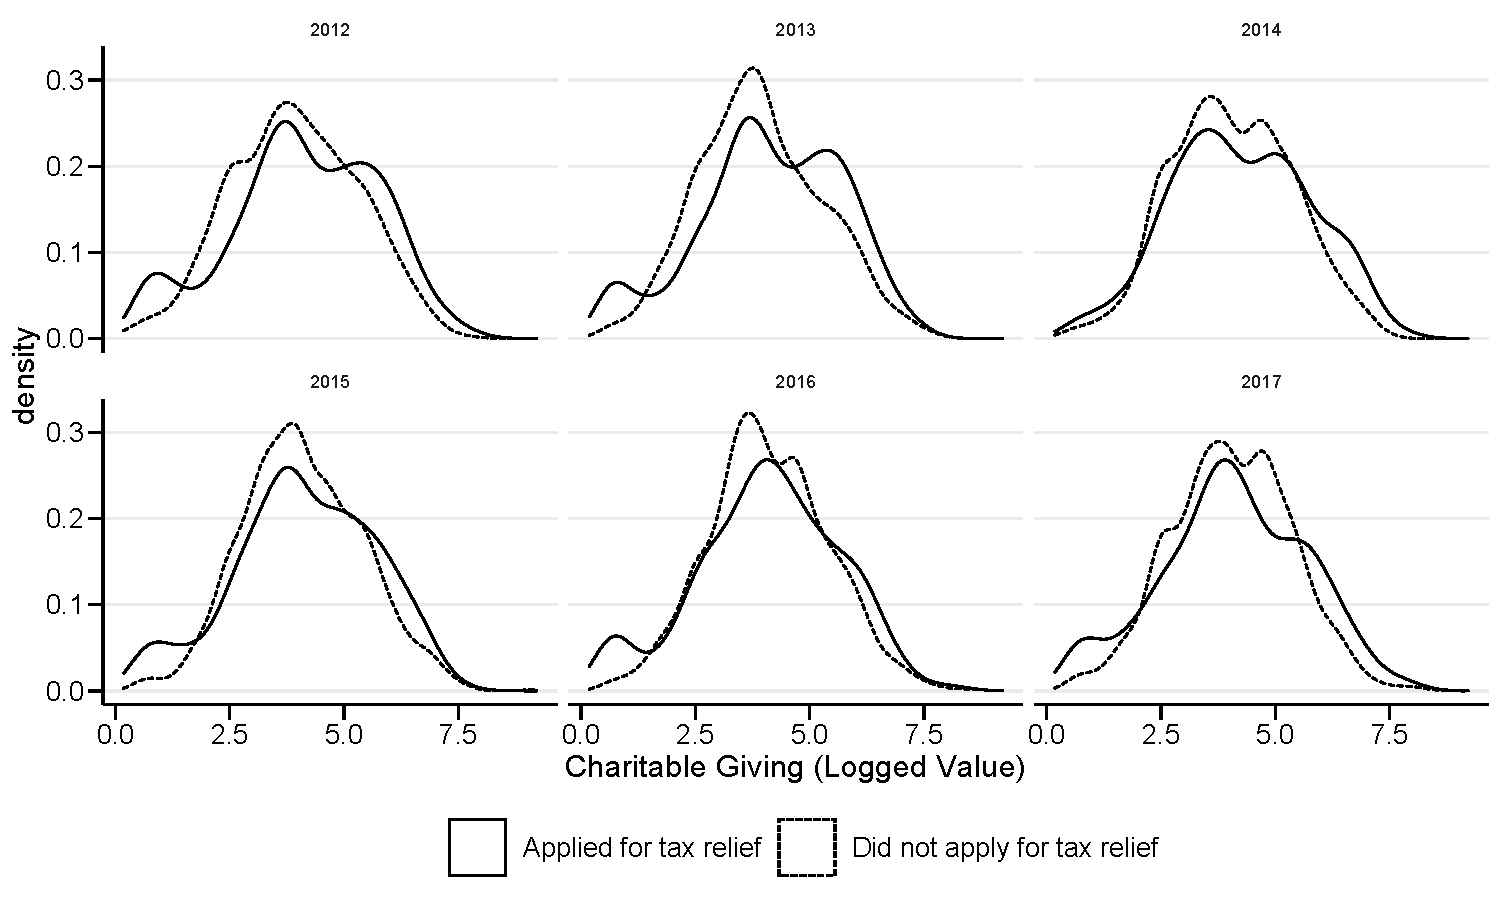
\includegraphics[width=0.7\linewidth,]{C:/Users/katoo/Desktop/NASTAB/paper/slide_files/figure-beamer/SummaryGivingIntensiveDist-1} 

}

\caption{Distribution of Charitable Giving among Those Who Donated}\label{fig:SummaryGivingIntensiveDist}
\end{figure}
\end{frame}

\begin{frame}{Share of Application Conditional on Donors by Wage Earners}
\protect\hypertarget{share-of-application-conditional-on-donors-by-wage-earners}{}
\begin{figure}[t]

{\centering 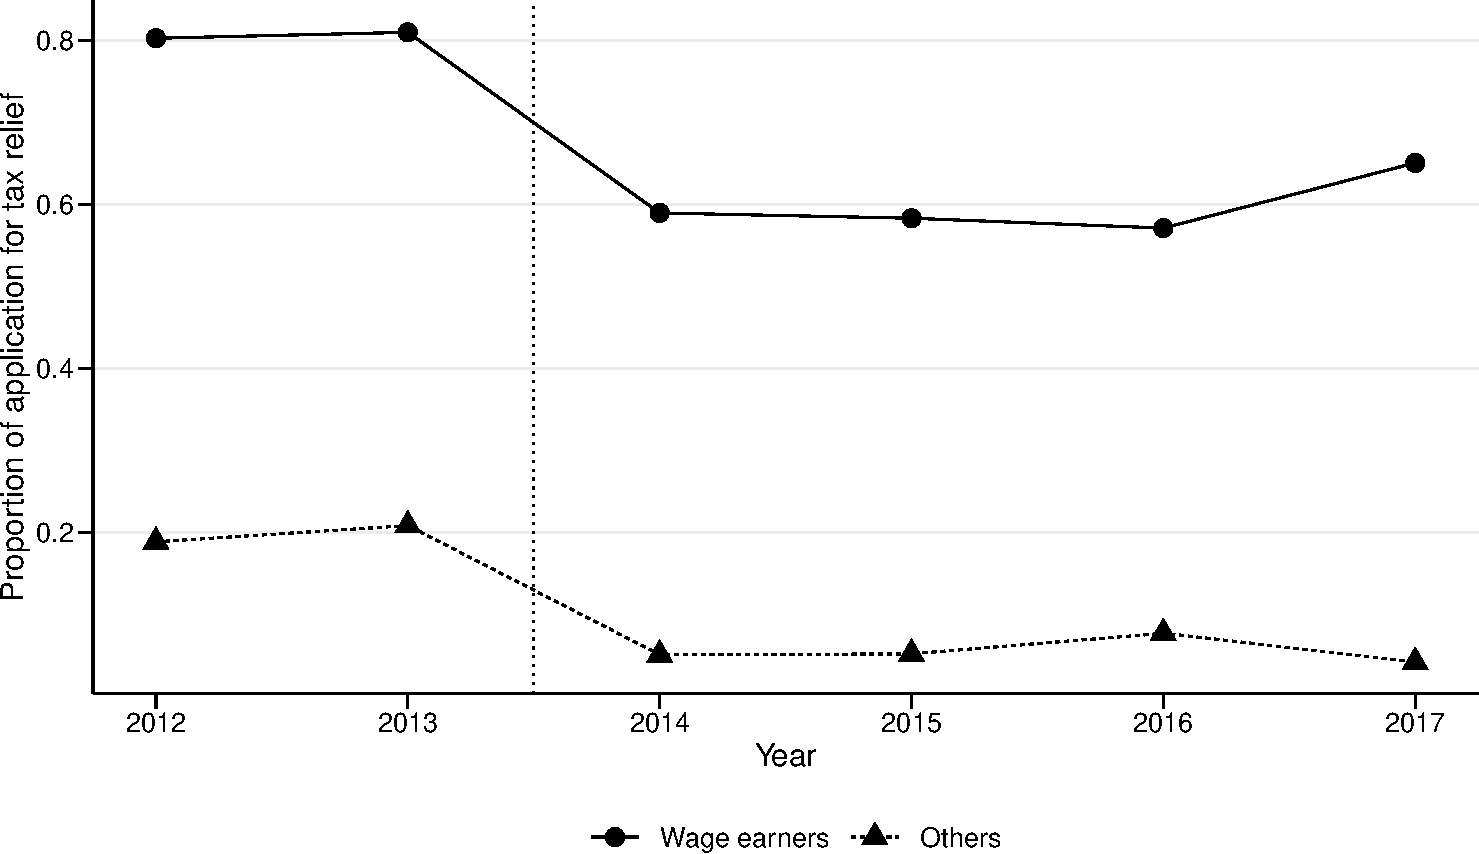
\includegraphics[width=0.7\linewidth,]{C:/Users/katoo/Desktop/NASTAB/paper/slide_files/figure-beamer/SummaryReliefbyEarner2-1} 

}

\caption{Share of Tax Relief by Wage Earners Conditional on Donors. Notes: A solid line is the share of applying for tax relief among wage eaners. A dashed line is the share of applying for tax relief other than wage earners.}\label{fig:SummaryReliefbyEarner2}
\end{figure}
\end{frame}

\begin{frame}{Price Elasticity Excluding Announcement Effect}
\protect\hypertarget{price-elasticity-excluding-announcement-effect}{}
\begin{table}

\caption{\label{tab:WoAnnoucementElasticity}Estimation of Last-Unit Price Elasticities Excluding 2013 and 2014 data}
\centering
\fontsize{7}{9}\selectfont
\begin{threeparttable}
\begin{tabular}[t]{lcccccc}
\toprule
\multicolumn{1}{c}{ } & \multicolumn{2}{c}{Overall} & \multicolumn{2}{c}{Intensive margin} & \multicolumn{2}{c}{Extensive margin} \\
\cmidrule(l{3pt}r{3pt}){2-3} \cmidrule(l{3pt}r{3pt}){4-5} \cmidrule(l{3pt}r{3pt}){6-7}
\multicolumn{1}{c}{ } & \multicolumn{1}{c}{FE} & \multicolumn{1}{c}{FE-2SLS} & \multicolumn{1}{c}{FE} & \multicolumn{1}{c}{FE-2SLS} & \multicolumn{1}{c}{FE} & \multicolumn{1}{c}{FE-2SLS} \\
\cmidrule(l{3pt}r{3pt}){2-2} \cmidrule(l{3pt}r{3pt}){3-3} \cmidrule(l{3pt}r{3pt}){4-4} \cmidrule(l{3pt}r{3pt}){5-5} \cmidrule(l{3pt}r{3pt}){6-6} \cmidrule(l{3pt}r{3pt}){7-7}
  & (1) & (2) & (3) & (4) & (5) & (6)\\
\midrule
log(last price) & -11.309*** & -6.331*** & -0.679** & -2.088*** & -3.097*** & -1.560***\\
 & (0.372) & (0.798) & (0.333) & (0.600) & (0.086) & (0.170)\\
\midrule
Implied price elasticity &  &  &  &  & -11.574*** & -5.830***\\
 &  &  &  &  & (0.320) & (0.634)\\
First-stage: log(first price) &  & 0.363 &  & 0.796 &  & 0.363\\
 &  & [244.3] &  & [270.6] &  & [244.3]\\
Num.Obs. & 20198 & 20198 & 5405 & 5405 & 20198 & 20198\\
FE: area & X & X & X & X & X & X\\
FE: indust & X & X & X & X & X & X\\
FE: pid & X & X & X & X & X & X\\
FE: year & X & X & X & X & X & X\\
Square of age & X & X & X & X & X & X\\
\bottomrule
\end{tabular}
\begin{tablenotes}
\item Notes: $^{*}$ $p < 0.1$, $^{**}$ $p < 0.05$, $^{***}$ $p < 0.01$. Standard errors are clustered at individual level. A square bracket is wald statistics of instrument.
\end{tablenotes}
\end{threeparttable}
\end{table}
\end{frame}

\begin{frame}{Subsample Analysis for Those Who Applied for Tax Relief}
\protect\hypertarget{subsample-analysis-for-those-who-applied-for-tax-relief}{}
\begin{table}

\caption{\label{tab:R1Elasticity}Estimating Intensive-Margin Price Elasticities for Those Who Applied for Tax Relief}
\centering
\fontsize{5}{7}\selectfont
\begin{threeparttable}
\begin{tabular}[t]{lcccc}
\toprule
  & (1) & (2) & (3) & (4)\\
\midrule
log(first price) & -1.203*** & -0.506 &  & \\
 & (0.390) & (0.847) &  & \\
log(last price) &  &  & -1.330*** & -0.254\\
 &  &  & (0.452) & (0.903)\\
log(income) & 0.525 & 6.126 & 0.532 & 6.093\\
 & (0.776) & (5.365) & (0.785) & (5.503)\\
1-year lag of price &  & 0.369 &  & 0.487\\
 &  & (0.884) &  & (0.911)\\
1-year lag of income &  & 1.040 &  & 1.129\\
 &  & (4.777) &  & (5.030)\\
1-year lead of income &  & -0.821 &  & -0.826\\
 &  & (0.907) &  & (0.904)\\
\midrule
Instrument: log(first price) &  &  & 0.942 & -0.000\\
 &  &  & [3083.6] & [0.0]\\
Num.Obs. & 4079 & 1029 & 3972 & 1024\\
FE: area & X & X & X & X\\
FE: indust & X & X & X & X\\
FE: pid & X & X & X & X\\
FE: year & X & X & X & X\\
Square of age & X & X & X & X\\
\bottomrule
\end{tabular}
\begin{tablenotes}
\item Notes: $^{*}$ $p < 0.1$, $^{**}$ $p < 0.05$, $^{***}$ $p < 0.01$. Standard errors are clustered at individual level. 1-year lead of price cannot be estimated because of collinearity.
\end{tablenotes}
\end{threeparttable}
\end{table}
\end{frame}

\begin{frame}{\(k\)-th Difference Model}
\protect\hypertarget{k-th-difference-model}{}
\begin{table}

\caption{\label{tab:KdiffElasticity}$k$-th Difference Model Using Those Who Applied for Tax Relief}
\centering
\fontsize{8}{10}\selectfont
\begin{threeparttable}
\begin{tabular}[t]{lccc}
\toprule
\multicolumn{1}{c}{ } & \multicolumn{1}{c}{1-year lag} & \multicolumn{1}{c}{2-year lag} & \multicolumn{1}{c}{3-year lag} \\
\cmidrule(l{3pt}r{3pt}){2-2} \cmidrule(l{3pt}r{3pt}){3-3} \cmidrule(l{3pt}r{3pt}){4-4}
  & (1) & (2) & (3)\\
\midrule
Difference of logged first price & -1.890* & -2.530*** & -4.057***\\
 & (1.107) & (0.895) & (0.720)\\
\midrule
First-stage: Instrument & 0.995 & 0.991 & 0.984\\
 & [34401.5] & [31041.1] & [17987.3]\\
Num.Obs. & 4014 & 3903 & 3765\\
FE: area & X & X & X\\
FE: indust & X & X & X\\
FE: year & X & X & X\\
Difference of square age & X & X & X\\
\bottomrule
\end{tabular}
\begin{tablenotes}
\item Notes: $^{*}$ $p < 0.1$, $^{**}$ $p < 0.05$, $^{***}$ $p < 0.01$. Standard errors are clustered at individual level. Instrument is difference between lagged first price in year $t$ and in year $t - k$ fixing income in year $t - k$.
\end{tablenotes}
\end{threeparttable}
\end{table}
\end{frame}

\begin{frame}{Heterogenous Price Elasticity in terms of Covariates}
\protect\hypertarget{heterogenous-price-elasticity-in-terms-of-covariates}{}
\begin{table}

\caption{\label{tab:CovHeteroElasticity}Heterogenous Last-Unit Price Elasticities in terms of Individual Characteristics}
\centering
\fontsize{8}{10}\selectfont
\begin{threeparttable}
\begin{tabular}[t]{lcccccc}
\toprule
\multicolumn{1}{c}{ } & \multicolumn{3}{c}{Intensive margin} & \multicolumn{3}{c}{Extensive margin} \\
\cmidrule(l{3pt}r{3pt}){2-4} \cmidrule(l{3pt}r{3pt}){5-7}
Covariate & Estimate & S.E. & N & Estimate & S.E. & N\\
\midrule
Female & -0.551 & (1.120) & 2921 & -9.786*** & (1.440) & 10674\\
Male & -1.919*** & (0.523) & 4313 & -5.126*** & (0.554) & 18022\\
University graduate & -2.048*** & (0.572) & 4723 & -4.494*** & (0.488) & 14778\\
High school graduate & -1.611 & (1.066) & 1977 & -10.300*** & (1.483) & 9803\\
Less than junior high school graduate & 1.012 & (1.467) & 534 & -23.121*** & (7.031) & 4115\\
Age < 40 & -1.538 & (1.459) & 1889 & -1.870 & (2.211) & 7800\\
40 $\le$ Age $\le$ 50 & -2.293*** & (0.781) & 2823 & -5.332*** & (0.627) & 9530\\
50 < Age & -0.714 & (0.718) & 2522 & -8.170*** & (1.214) & 11366\\
Wage earner & -1.966*** & (0.486) & 5517 & -2.009*** & (0.451) & 15596\\
Non wage earner & -11.226 & (11.177) & 1690 & -21.142 & (33.822) & 12934\\
\bottomrule
\end{tabular}
\begin{tablenotes}
\item Notes: $^{*}$ $p < 0.1$, $^{**}$ $p < 0.05$, $^{***}$ $p < 0.01$. Standard errors are clustered at individual level.
\end{tablenotes}
\end{threeparttable}
\end{table}
\end{frame}

\begin{frame}{Heterogenous Price Elasticity in terms of Organization Type}
\protect\hypertarget{heterogenous-price-elasticity-in-terms-of-organization-type}{}
\begin{table}

\caption{\label{tab:TypeHeteroElasticity}Estimating Last-Unit Price Elasticities for Each Oraganization Type}
\centering
\fontsize{8}{10}\selectfont
\begin{threeparttable}
\begin{tabular}[t]{lcccccc}
\toprule
\multicolumn{1}{c}{ } & \multicolumn{3}{c}{Intensive margin} & \multicolumn{3}{c}{Extensive margin} \\
\cmidrule(l{3pt}r{3pt}){2-4} \cmidrule(l{3pt}r{3pt}){5-7}
Type & Estimate & S.E. & N & Estimate & S.E. & N\\
\midrule
Social welfare & -1.814** & (0.867) & 2990 & -5.514*** & (1.394) & 28696\\
Education & 1.805 & (4.507) & 178 & 14.633* & (7.644) & 28696\\
Political party & 17.955 & (47.747) & 258 & 20.448*** & (7.071) & 28696\\
Religious institution & -1.300** & (0.619) & 3867 & -4.436*** & (1.040) & 28696\\
Relief activities by religious institution & -4.985 & (3.092) & 532 & -2.378 & (4.125) & 28696\\
Others & -3.847 & (3.780) & 422 & 2.706 & (4.644) & 28696\\
Culture &  &  &  & 15.386 & (10.951) & 28696\\
\bottomrule
\end{tabular}
\begin{tablenotes}
\item Notes: $^{*}$ $p < 0.1$, $^{**}$ $p < 0.05$, $^{***}$ $p < 0.01$. Standard errors are clustered at individual level. We cannot the intensive-margin price elasticity for donations for culture due to small sample.
\end{tablenotes}
\end{threeparttable}
\end{table}
\end{frame}

\hypertarget{references}{%
\section*{References}\label{references}}
\addcontentsline{toc}{section}{References}

\begin{frame}{References}
\hypertarget{refs}{}
\begin{CSLReferences}{1}{0}
\leavevmode\vadjust pre{\hypertarget{ref-Almunia2020}{}}%
Almunia, M., Guceri, I., Lockwood, B., Scharf, K., 2020. More giving or more givers? The effects of tax incentives on charitable donations in the UK. Journal of Public Economics 183. doi:\href{https://doi.org/10.1016/j.jpubeco.2019.104114}{10.1016/j.jpubeco.2019.104114}

\end{CSLReferences}
\end{frame}

\end{document}
